\section{Data and Methods}
\label{sec:data_methods}

\subsection{Data and calendar construction}

The analysis combines daily-source-frequency prices for cocoa, gold, Brent crude oil and WTI crude oil from Yahoo Finance with the Ghanaian cedi exchange rate from the Bank of Ghana. Returns begin in January 2015. The cedi is signed so that positive returns denote appreciation and negative returns denote depreciation.

Two co-equal calendar constructions are retained. Panel A imposes a business-day calendar, carries missing prices forward for at most three business days, and then computes log returns. It contains 3,008 returns from 5 January 2015 to 15 July 2026. Panel B restricts the data to dates on which all five series have actual observations and computes returns between consecutive common dates. It contains 2,774 returns from 5 January 2015 to 10 July 2026. Panel B intervals range from one to six calendar days, with a median of one day. The two constructions therefore make different compromises: Panel A preserves nominal business-day frequency but can create carried-price zero returns, whereas Panel B removes forward-filled returns but does not represent a fixed 24-hour horizon.

\begin{figure}[htbp]
\centering
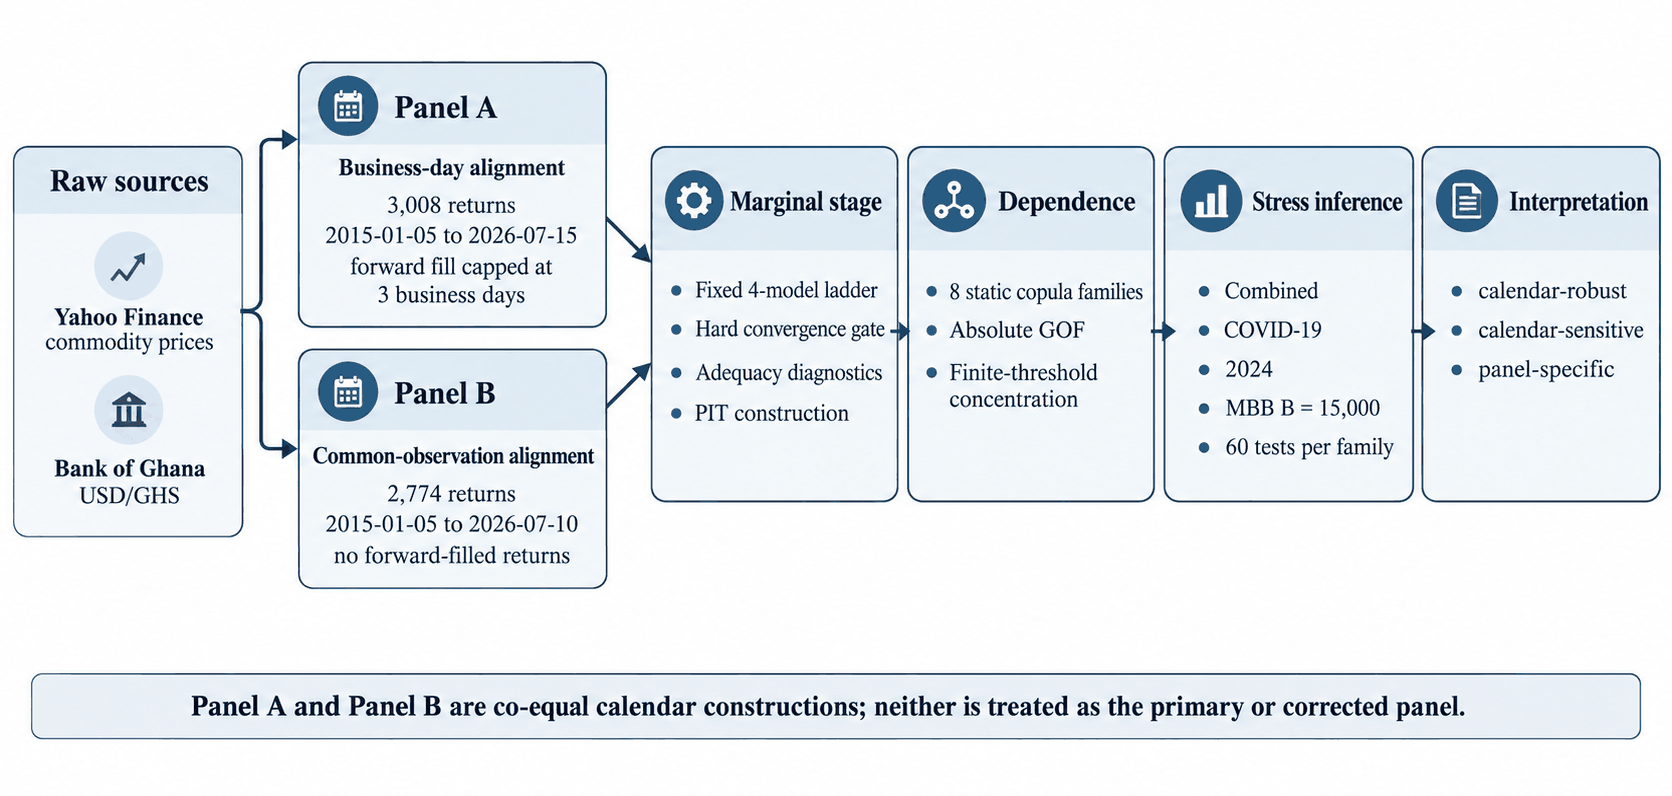
\includegraphics[width=0.98\linewidth]{figures/figure_01_calendar_workflow.png}
\caption{Data and calendar-construction workflow. Panel A uses business-day alignment with forward filling capped at three business days, whereas Panel B uses consecutive common actual-source dates without forward-filled returns.}
\label{fig:calendar-workflow}
\end{figure}

\begin{table}[htbp]
\centering
\caption{Calendar construction summary.}
\label{tab:calendar-summary}
\small
\begin{tabularx}{\textwidth}{lXX}
\toprule
\textbf{Feature} & \textbf{Panel A} & \textbf{Panel B} \\
\midrule
Alignment & Business-day grid & Common actual-source dates \\
Return observations & 3,008 & 2,774 \\
Return period & 5 Jan 2015--15 Jul 2026 & 5 Jan 2015--10 Jul 2026 \\
Missing-price rule & Forward fill, maximum 3 business days & No forward-filled return observations \\
Return interval & Nominal business-day & Previous common observation date \\
Exact Cedi zero-return share & 22.27\% & 16.51\% \\
Role in analysis & Co-equal specification & Co-equal specification \\
\bottomrule
\end{tabularx}
\end{table}

The WTI settlement of \(-37.630001\) on 20 April 2020 requires special treatment because a standard log return is undefined at a non-positive price. Panel A does not use that raw value directly in the log-return calculation and shifts the associated price movement to the next positive observation. Panel B drops the common interval affected by the non-positive value. The episode is retained as a documented data limitation rather than forced into an invalid logarithmic transformation.

Exact zero returns are materially more common in Panel A because of forward filling. For the cedi, however, the zero share remains high even in Panel B (16.51\%), indicating that the zero-heavy daily process is not solely an artifact of the business-day construction. This feature becomes important in the marginal-model diagnostics.

\subsection{Marginal filtering and pseudo-observations}

Each return series is filtered with a fixed four-model ladder: AR(1)-GJR-GARCH(1,1)-t, AR(2)-GJR-GARCH(1,1)-t, AR(1)-EGARCH(1,1)-t, and AR(1)-GJR-GARCH(1,1)-skew-t. A fit is eligible only if the optimizer converges and the likelihood, parameters, standardized residuals, conditional volatilities and probability-integral-transform (PIT) values are finite. Adequacy is assessed at the 5\% level using Ljung--Box tests on standardized residuals and squared standardized residuals (10 lags) and a Kolmogorov--Smirnov test of PIT values against Uniform(0,1). The first valid adequate model in the fixed ladder is selected. If none passes, the converged candidate with the lowest AIC is retained only as an inadequate reference model.

For a selected marginal model, standardized residuals are mapped through the fitted innovation distribution and then converted to rank-based pseudo-observations,
\[
u_t=\frac{\operatorname{rank}(\tilde u_t)}{n+1}.
\]
PIT values are clipped to \([10^{-6},1-10^{-6}]\) for numerical stability. A separate audit of the resulting Panel A cedi tie shows that restoring the underlying order changes no prespecified tail-set membership and produces only negligible changes in observed cedi-pair goodness-of-fit statistics.

\subsection{Copula specification and absolute goodness of fit}

With five series there are ten unordered pairs. Each pair is fitted with eight static bivariate copula families: Gaussian, Student-t, Clayton, Gumbel, Frank, Joe, survival Clayton and survival Gumbel. AIC is retained only as a relative-fit descriptor. Absolute adequacy is evaluated separately using a Rosenblatt-transform Cram\'{e}r--von Mises statistic with parametric bootstrap.

For fitted copula \(C_{\hat\theta}\), the Rosenblatt transformation is
\[
e_{1i}=u_i,\qquad e_{2i}=h_{\hat\theta}(v_i\mid u_i),
\]
and the transformed empirical distribution is compared with the product-uniform reference over a 50 by 50 grid. Each bootstrap replicate is simulated from the fitted family, re-ranked, re-estimated and retested. The Monte Carlo p-value is
\[
\hat p=\frac{1+\sum_{b=1}^{B} I\{S_n^{(b)}\ge S_n\}}{B+1}.
\]
All 80 pair-family cells are first evaluated with \(B=2000\); cells with initial \(0.03\le\hat p\le0.07\) are rerun with \(B=5000\). Rejection at 5\% is interpreted as evidence that the tested static family is inadequate under the implemented procedure. Non-rejection is not treated as proof that the family is the true model.

\subsection{Finite-threshold tail concentration and stress inference}

For pseudo-observations \((u_i,v_i)\), lower- and upper-tail concentration are measured at \(q\in\{0.025,0.05,0.10\}\):
\[
\hat\lambda_L(q)=\frac{1}{nq}\sum_{i=1}^{n}I(u_i\le q,v_i\le q),\qquad
\hat\lambda_U(q)=\frac{1}{nq}\sum_{i=1}^{n}I(u_i\ge 1-q,v_i\ge 1-q).
\]
These are finite-threshold concentration measures and are not described as asymptotic tail-dependence coefficients.

Stress--calm differences are evaluated under three prespecified stress definitions: COVID-19 (1 March--30 June 2020), calendar year 2024, and their union (Combined). For each definition, ten pairs, three thresholds and two tails produce 60 simultaneous tests. Inference uses a moving-block bootstrap with block length 20 and \(B=15{,}000\) replicates. Nominal p-values are reported descriptively, but confirmatory interpretation uses both Bonferroni family-wise-error control and Benjamini--Hochberg false-discovery-rate control within each 60-test family.

\subsection{Extreme-value and cedi diagnostics}

Extreme-value diagnostics use the loss transform of standardized residuals, \(L_t=-\hat z_t\), with a peaks-over-threshold generalized Pareto model above the empirical 90th percentile. The analysis records the GPD shape and scale parameters, 99\% VaR and expected shortfall, and threshold sensitivity. Because the cedi marginal fails the adequacy gate in both panels, cedi EVT estimates are interpreted only conditionally on the retained reference residual process.

Supplementary diagnostics examine cedi threshold sensitivity, alternative cedi treatments and the numerical effect of PIT clipping. These analyses are supporting checks rather than additional headline specifications.

\subsection{Use of generative artificial intelligence}

During manuscript preparation, the author used OpenAI's ChatGPT (GPT-5.6 Sol) to assist with code review, manuscript organization, language editing, consistency checking and preparation of publication materials. All analyses, numerical results, interpretations, references and final manuscript content were reviewed and verified by the author, who takes full responsibility for the work.
